\documentclass[10pt]{amsart}
\usepackage{amsmath,amssymb,amsthm,mathtools,mathrsfs}
\usepackage[a4paper,hmargin=0.76in,vmargin=0.60in]{geometry}
\usepackage{booktabs}
\usepackage{array}
\usepackage{tabularx}
\usepackage{tikz}
\usetikzlibrary{positioning,arrows.meta,fit}
\usepackage[hypertexnames=false]{hyperref}
\hypersetup{hidelinks}
\usepackage[final,expansion=false]{microtype}
\usepackage{url}
\emergencystretch=2.5em

\newtheorem{theorem}{Theorem}[section]
\newtheorem{proposition}[theorem]{Proposition}
\newtheorem{lemma}[theorem]{Lemma}
\newtheorem{corollary}[theorem]{Corollary}
\theoremstyle{definition}
\newtheorem{definition}[theorem]{Definition}
\theoremstyle{remark}
\newtheorem{remark}[theorem]{Remark}

\newcommand{\C}{\mathbb C}
\newcommand{\R}{\mathbb R}
\newcommand{\Z}{\mathbb Z}
\newcommand{\Q}{\mathbb Q}
\newcommand{\F}{\mathbb F}
\newcommand{\Rel}{\operatorname{Re}}
\newcommand{\Iml}{\operatorname{Im}}
\newcommand{\Frob}{\mathrm{Frob}}
\newcommand{\Tl}{T_{\lim}}
\newcommand{\Il}{I_{\lim}}
\newcommand{\U}{\mathrm U}
\newcommand{\cT}{\mathcal T}
\newcommand{\cS}{\mathcal S^{\mathrm{ram}}}
\newcommand{\cSi}{\mathcal S^{\mathrm{ram}}_{\mathrm{int}}}
\newcommand{\cL}{\mathcal L_D}
\newcommand{\dT}{d_{\mathcal T}}
\newcommand{\hmain}{h_{\mathrm{main}}}
\newcommand{\rem}{\mathrm{rem}}
\newcommand{\Pa}{\mathsf P_a}
\newcommand{\Pb}{\mathsf P_b}
\newcommand{\Pl}{\mathsf P}
\newcommand{\pp}{\mathfrak p}
\newcommand{\Gbar}{\overline G}
\newcolumntype{Y}{>{\raggedright\arraybackslash}X}

\begin{document}
\addtolength{\abovedisplayskip}{-2pt}
\addtolength{\belowdisplayskip}{-2pt}
\title[The Riemann hypothesis along the rows of Weil's proof]{The Riemann hypothesis along the rows of Weil's proof:\\ a guide to the series}
\author{David Alejandro Trejo Pizzo}
\date{}
\begin{abstract}
Weil's proof of the Riemann hypothesis for a curve over a finite field has four steps: the ring
of correspondences with its intersection pairing, the Frobenius correspondences, the trace
formula, and the index inequality. A series of twelve papers carries these four steps, row by
row, to $\operatorname{Spec}\mathbb Z$. We describe its logical chain for a reader who has opened
none of them: what replaces each row over $\mathbb Z$, what each paper establishes, how the
index inequality becomes the sign of a Hermitian form on functions supported in an interval,
and how that sign is obtained, through a one-sided criterion for a sum over primes and three
theorems on integral algebraic modular forms, from the absence of zeros of Dirichlet
$L$-functions in $\Re s>\tfrac12$.
\end{abstract}
\maketitle

\section{Introduction}\label{sec:intro}
Let $C$ be a smooth projective curve over a finite field $\F_q$. Weil's proof that the zeros of
its zeta function lie on the line $\Rel s=\tfrac12$ takes place on the surface $C\times C$
\cite{Weil1948}. It uses four things: the divisor classes on the surface, which are the
correspondences of the curve and carry a product, a transpose and an intersection pairing; the
graphs of the powers of the Frobenius endomorphism; the formula that expresses the intersection
number of such a graph with the diagonal through the eigenvalues of Frobenius; and an
inequality for the self-intersection of a correspondence. The first three are constructions and
identities. The fourth is a statement of positivity, and it is the one that bounds the eigenvalues.

The question of whether this argument can be carried to the field $\Q$ is old, and its
difficulties are well known: there is no surface
$\operatorname{Spec}\Z\times\operatorname{Spec}\Z$ on which to intersect, and no Frobenius.
What does exist is the right-hand side of the argument. Weil's explicit formula \cite{Weil52}
has the shape of the trace formula, with the zeros of $\zeta$ in the place of the eigenvalues,
and Weil observed that the Riemann hypothesis is equivalent to the positivity of the
distribution it defines. Connes \cite{Connes99} obtained the local terms of the explicit formula
from a trace formula on the adele class space attached to a finite set of places, and Connes,
Consani and Marcolli \cite{CCM} read them as intersection numbers with the diagonal.

The series described here follows that line, in the most literal way available: it goes through
the four steps of Weil's proof, which we call Rows~A, B, C and~D, and supplies for each an
object or a statement over $\Q$ that occupies the same place. Rows~A, B and~C are the papers
\cite{P43}, \cite{P44} and \cite{Paper45}; they build the correspondences, their algebra, a
trace and a Hermitian form on the semilocal idele class groups, a family of measures that composes
like the powers of Frobenius and meets the diagonal in $\Lambda(n)/\sqrt n$, and the evaluation
of the trace as Weil's explicit formula. Row~D is the paper \cite{P46}, together with eight companion
papers \cite{P49}--\cite{P56}. It treats the index inequality, which for these objects is the
statement that a certain Hermitian form on functions supported in an interval $(-T,T)$ has a
definite sign for every $T$; this statement is equivalent to the Riemann hypothesis, and
\cite{P46} proves it.

The four rows are of two kinds, as they are for a curve. Rows~A--C are a framework. They
contain theorems, some of them of independent interest, but none of these says anything about
the location of a zero, and they were not expected to: for a curve, too, the first three steps
hold for formal reasons and the whole difficulty is in the fourth. Row~D is where a
positivity statement must be proved, and there the geometry of a surface gives no help, since
the Hodge index theorem has no known counterpart for the objects of Rows~A--C. The proof of the
sign in \cite{P46} therefore goes another way. It shows that no Dirichlet $L$-function
vanishes in $\Rel s>\tfrac12$, and the sign follows from the explicit formula. The absence of
zeros is obtained from a bound, on one side only, for a sum over primes; and that bound comes
from three theorems on integral algebraic modular forms on unitary groups over a CM field,
the Short Forms Theorem, the Spanning Theorem and the Covolume Theorem. They are our way of
organising, as ordinary mathematics, the argument of L.~Alpoge (see
Section~\ref{sec:conclusion}); their proofs occupy the eight companion papers. The whole of
Row~D is the chain
\[
\text{three theorems}\ \Longrightarrow\ \text{main inequality}\ \Longrightarrow\
\text{one-sided bound}\ \Longrightarrow\ \text{criterion}\ \Longrightarrow\ \mathrm{GRH}
\ \Longrightarrow\ \mathrm{RH},
\]
in which each arrow is a short argument and all the weight lies in the three theorems.

Table~\ref{tab:rows} summarises the correspondence between the two situations. Section~\ref{sec:weil}
recalls Weil's argument in the form of four rows. Section~\ref{sec:ABC} describes Rows~A--C,
and Section~\ref{sec:D} the form whose sign is Row~D and its equivalence with the Riemann
hypothesis. Sections~\ref{sec:criterion}--\ref{sec:squeeze} follow the proof of the sign: the
criterion, the arithmetic data, the three theorems, and the inequality that results from them.
Section~\ref{sec:companions} says where each companion paper enters, and
Section~\ref{sec:order} gives the dependencies between the papers and an order in which to read them.
We state results in simplified form whenever the exact statement requires notation that would
take pages to set up; in each such case we say so and name the exact statement.

\begin{table}[h]
\small
\begin{tabularx}{\textwidth}{@{}l>{\hsize=.86\hsize}Y>{\hsize=1.14\hsize}Yl@{}}
\toprule
Row & Curve $C$ over $\F_q$ & $\operatorname{Spec}\Z$ & Paper\\
\midrule
A & Correspondences on $C\times C$: product, transpose, intersection pairing, the two rulings and the bidegree
  & Graph bimodules of idele classes; the test algebra $C_c^\infty(C_S)$ with convolution and involution; the trace $T$ and the form $T(F\star G^\dagger)$; the two Tate functionals & \cite{P43}\\
B & Graphs of the powers of Frobenius; their intersection with the diagonal counts points
  & Measures $\Frob_n$ with $\Frob_m\star\Frob_n=\Frob_{mn}$; contact with the diagonal $\Lambda(n)/\sqrt n$ & \cite{P44}\\
C & Trace formula: $\Delta\cdot\Gamma_{n}=1+q^n-\sum_i\alpha_i^n$
  & Weil's explicit formula: $\Tl(\Gamma_h)=\Phi_h(0)+\Phi_h(1)-\sum_\rho\Phi_h(\rho)$ & \cite{Paper45}\\
D & Index inequality: $D\cdot D\le 2d_1d_2$
  & Sign of the radial form on every window $(-T,T)$; equivalent to the Riemann hypothesis & \cite{P46}, \cite{P49}--\cite{P56}\\
\bottomrule
\end{tabularx}
\medskip
\caption{The four rows.}\label{tab:rows}
\end{table}

\section{Weil's proof for a curve, in four rows}\label{sec:weil}
We recall the argument in the form that the series transposes. Let $g$ be the genus of $C$ and
$X=C\times C$.

\emph{Row A: the objects.} A correspondence is a divisor class on $X$. Correspondences compose,
the exchange of the two factors gives a transpose $D\mapsto D^{t}$, and there is an intersection
pairing $D\cdot D'$; the diagonal $\Delta$ is the unit for composition, and
$D\cdot D'=\Delta\cdot(D\circ D'^{\,t})$, so that the pairing is determined by a single
functional, the intersection number with the diagonal. The two rulings $C\times\{\mathrm{pt}\}$
and $\{\mathrm{pt}\}\times C$ have self-intersection $0$ and meet once: they span a hyperbolic
plane. The intersection numbers $d_1,d_2$ of $D$ with them form its bidegree, and $D$ is the sum
of a combination of the rulings and a \emph{primitive} part $P$, orthogonal to both, so that
\begin{equation}\label{eq:decomp}
 D\cdot D'=P\cdot P'+d_1d_2'+d_2d_1' .
\end{equation}

\emph{Row B: the Frobenius family.} The graph $\Gamma_n$ of the $n$-th power of the Frobenius
endomorphism is a correspondence whose two degrees are $1$ and $q^n$, one has
$\Gamma_m\circ\Gamma_n=\Gamma_{m+n}$, and $\Delta\cdot\Gamma_n$ is the number $N_n$ of points of
$C$ over $\F_{q^n}$.

\emph{Row C: the trace formula.} If $\alpha_1,\dots,\alpha_{2g}$ are the inverse roots of the
numerator of the zeta function of $C$, then $\Delta\cdot\Gamma_n=1+q^n-\sum_i\alpha_i^n$. The
terms $1$ and $q^n$ come from the rulings and the sum from the primitive part.

\emph{Row D: the index inequality.} The pairing is negative semidefinite on primitive classes:
$P\cdot P\le0$, or, by \eqref{eq:decomp}, $D\cdot D\le2d_1d_2$ for every correspondence. This is
the inequality of Castelnuovo and Severi, which Weil proved in arbitrary characteristic
\cite{Weil1948}; it is also a consequence of the Hodge index theorem on the surface $X$. Apply it
to $D=a\Delta+b\Gamma_n$, whose degrees are $a+b$ and $a+bq^n$. Since $\Delta\cdot\Delta=2-2g$ and
$\Gamma_n\cdot\Gamma_n=q^n(2-2g)$, it gives
$2ab\,(N_n-1-q^n)\le2g\,(a^2+q^nb^2)$ for all integers $a,b$; so the quadratic form
$g\,a^2+ab\sum_i\alpha_i^n+g\,q^nb^2$ is nowhere negative, and
$|\sum_i\alpha_i^n|\le2g\,q^{n/2}$. This holds for all $n$, whence $|\alpha_i|\le\sqrt q$ for
every $i$, and $|\alpha_i|=\sqrt q$ because the functional equation permutes the $\alpha_i$ by
$\alpha\mapsto q/\alpha$.

Three features of this argument guide what follows. The pairing is recovered from a trace and
an involution, so that over $\Q$ it suffices to have an algebra with an involution and a linear
functional on it. The two rulings, which are not primitive and on which the pairing is
hyperbolic, must be found and split off before any sign can be asked for. And on the
combinations of the graphs $\Gamma_n$ and their transposes the inequality of Row~D is
equivalent, given Rows~A--C, to the statement on the eigenvalues: there it is another form of the
Riemann hypothesis for the curve, which on a surface happens to have a geometric proof.

\section{Rows A, B and C: the framework over \texorpdfstring{$\operatorname{Spec}\mathbb Z$}{Spec Z}}\label{sec:ABC}
\subsection{Row A: correspondences, the trace and the form}
Fix a finite set $S$ of places of $\Q$ containing $\infty$ and at least one prime, and write
$S_f=S\smallsetminus\{\infty\}$. Let $A_S=\R\times\prod_{p\in S_f}\Q_p$ and let $\Gamma_S$ be the
group of positive rationals whose factorisation involves only the primes of $S_f$. The group
that takes the place of the curve is the semilocal idele class group
\[
 C_S=\Gamma_S\backslash A_S^\times\ \cong\ \R^\times\times\prod_{p\in S_f}\Z_p^\times ,
\]
with its modulus $|\cdot|_S$ and the homomorphisms $j_v\colon\Q_v^\times\to C_S$, $v\in S$. The
paper \cite{P43} does two things on it, which are logically independent.

The first gives a meaning to the word correspondence. An idele $a\in A_S^\times$ acts by
dilation, and the graph of this dilation is realised as a bimodule $E_a$ over the crossed
product $U$ of an algebra of functions on $\R^\times\times\prod_{p\in S_f}\Q_p$ by $\Gamma_S$:
it is $U$ itself, with the right action twisted by the dilation. These bimodules compose as
graphs do, $E_a\widehat\otimes_UE_b\cong E_{ab}$; $E_a$ and $E_b$ are isomorphic if and only if
$a$ and $b$ have the same class in $C_S$; and $a\mapsto a^{-1}$ gives an involution. Families of
them with coefficients in the test algebra $C_c^\infty(C_S)$ compose by convolution: with
$F^\dagger(u)=\overline{F(u^{-1})}$, the algebra $(C_c^\infty(C_S),\star,\dagger)$ is the algebra
of correspondences. The Hochschild complex of $U$ with coefficients in $E_a$ is graded by
$\Gamma_S$, and each graded part is computed up to homotopy equivalence: it is an exterior
algebra on $|S_f|$ generators with zero differential, to which, in at most one degree, two
copies of a Koszul complex are added, whose homology the paper does not compute.

The second is the intersection number. On the test algebra one considers the functional
\begin{equation}\label{eq:trace}
 T(F)=\sum_{v\in S}W_v(F)+c\,F(1),\qquad
 W_v(F)=\int_{\Q_v^\times}' F(j_v(x))\,\frac{|x|_v^{1/2}}{|1-x|_v}\,d^*x ,
\end{equation}
in which the $W_v$ are the local terms of Weil's explicit formula, in the form given by Connes
\cite[Appendix~II]{Connes99}, the prime on the integral denotes a regularisation at $x=1$, and
$c$ is a real constant, which nothing in the construction fixes: two regularisations that involve
no derivative of $F$ at the identity differ by a multiple of $F(1)$. The functional $T$ stands in
the place of the intersection number with the diagonal, and
\[
 I_A(F,G)=T(F\star G^\dagger)
\]
in the place of the intersection pairing. The two characters of the algebra
$\lambda_\mp(F)=\int_{C_S}F(u)\,|u|_S^{\mp1/2}\,d^*u$, which we call the Tate functionals, stand in
the place of the two degrees $d_1,d_2$; a function is \emph{primitive} if both vanish on it.
For a fixed $S$ the paper determines what is true of these objects. The Fourier transform of
$\sum_vW_v$ on the dual group of $C_S$ is computed in closed form; it is bounded above, with an
explicit supremum $m>0$, and its analytic continuation has simple poles at the two characters
$|\cdot|_S^{\pm1/2}$, which is where the Tate functionals are read. The form $I_A$ is
nondegenerate for every $c$. It has infinite negative index for every $c$, and infinite positive
index if and only if $c>-m$; for $c\le-m$ it is negative definite. In particular for $c=0$, the
value that Row~C requires, the form has no sign for a fixed $S$, and the same holds for its
restriction to the primitive functions. The rulings are not test functions: they exist as two elements
of a completion of the algebra, on which the algebra acts through $\lambda_+$ and $\lambda_-$,
and the form does not extend continuously to them. Finally, when $S$ grows the trace of a given
function changes by finitely many terms and then stabilises; this defines $\Tl$ and
$\Il$ on the union of the test algebras. In the limit the pairing of the two rulings is
recovered along radial approximations $F_n$, $G_m$ with slowly varying profiles: by Mertens'
theorem $\Il(F_n,G_m)=1+O(\max(n,m)^{-1})$, the value it has on a surface, while
$\Il(F_n,F_n)$ and $\Il(G_m,G_m)$ tend to $0$. Other approximations of the rulings give
other limits.

\subsection{Row B: the Frobenius family}
For every integer $n\ge1$ whose prime divisors lie in $S$, the paper \cite{P44} defines a
probability measure $\Frob_n$ on $C_S$, the Haar measure of a coset of a compact subgroup, such
that
\[
 \Frob_m\star\Frob_n=\Frob_{mn},
\]
and such that $\Frob_n$ determines $n$. This family takes the place of the graphs of the powers
of Frobenius, the multiplicative monoid of the integers replacing the additive monoid of the
exponents. The measures $\Frob_n$ are not test functions, and the trace is computed on test
functions $\Frob_n^{[h,N]}$ that approximate them, where $N\ge1$ is a level and $h$ a profile in
the archimedean coordinate. For $n\ge2$, if the support of $h$ lies in an interval contained in
$(n^{-2},1)$ that contains no integral power of a prime of $S$ other than $1/n$, the finite places give
\begin{equation}\label{eq:contact}
 \sum_{p\in S_f}W_p\bigl(\Frob_n^{[h,N]}\bigr)=\Lambda(n)\,n^{-1/2}\,h(1/n),
\end{equation}
with $\Lambda$ the von Mangoldt function. Thus on these functions the family meets the diagonal
exactly at the prime powers, with multiplicity $\log p$ and the normalising factor $n^{-1/2}$,
as the Frobenius correspondences contribute the numbers of points; when $n$ has two distinct
prime divisors the support of $\Frob_n$ meets none of the subgroups $j_p(\Q_p^\times)$ and the
contact is zero. The coefficients $(\log p)\,p^{-k/2}$ are those of the explicit formula; what
is added is a family of measures that composes according to a law, with approximating test
functions on which the trace produces these coefficients. The coefficient belongs to the
functions $\Frob_n^{[h,N]}$ and is not a value of $T$ at the measure, to which $T$ does not
extend by weak continuity.

Averaging $\Frob_n$ over the maximal compact subgroup of $C_S$ gives the Haar measure of the
level set $|u|_S=1/n$, and this \emph{radial} family makes sense for every positive real
parameter. Radial functions are those of the form $\Gamma_h(u)=h(-\log|u|_S)$ with
$h\in C_c^\infty(\R)$; they form a subalgebra, and for $0\notin\operatorname{supp}h$
\begin{equation}\label{eq:radtrace}
 T(\Gamma_h)=\sum_{p\in S_f}\sum_{k\ge1}\frac{\log p}{p^{k/2}}\bigl[h(k\log p)+h(-k\log p)\bigr]
 +\int_{\R}\frac{e^{-|t|/2}}{1-e^{-2|t|}}\,h(t)\,dt .
\end{equation}
The paper also computes the form $I_A$ on both families, and attaches to each integer $n>1$ a
complex of abelian groups whose cohomology has order $e^{\Lambda(n)}$; no map is constructed
between this complex and the trace.

\subsection{Row C: the explicit formula}
The right-hand side of \eqref{eq:radtrace} is the arithmetic side of Weil's explicit formula
restricted to the primes of $S$. The paper \cite{Paper45} identifies the limit over $S$. For
$h\in C_c^\infty(\R)$ put
\[
 \Phi_h(s)=\int_{\R}h(t)\,e^{(s-\frac12)t}\,dt ,
\]
and let $\rho$ run over the zeros of $\xi(s)=\tfrac12s(s-1)\pi^{-s/2}\Gamma(s/2)\zeta(s)$, with
multiplicity. With the normalisation of the regularisation fixed in Row~A and $c=0$,
\begin{equation}\label{eq:EF}
 \Tl(\Gamma_h)=\Phi_h(0)+\Phi_h(1)-\sum_\rho\Phi_h(\rho) ,
\end{equation}
the sum being absolutely convergent; for a finite $S$ the same identity holds as soon as $h$
vanishes outside $(-\log\ell,\log\ell)$, $\ell$ the least prime not in $S$. The formula holds for
no other value of $c$. This is Weil's explicit formula \cite{Weil52}, proved in \cite{Paper45}
in the required normalisation, and it is the trace formula of Row~C: the two terms
$\Phi_h(0)$ and $\Phi_h(1)$ are the Tate functionals $\lambda_+(\Gamma_h)$ and
$\lambda_-(\Gamma_h)$, which arise as the residues at $s=0$ and $s=1$ of a contour integral, in
the place of $1$ and $q^n$, and the sum over the zeros is the primitive part. Polarising, for
$F,G\in C_c^\infty(\R)$,
\begin{equation}\label{eq:EFform}
 \Il(\Gamma_F,\Gamma_G)=\beta\bigl(M(\Gamma_F),M(\Gamma_G)\bigr)-\sum_\rho\Phi_F(\rho)\,\overline{\Phi_G(1-\bar\rho)} ,
\end{equation}
where $M=(\lambda_-,\lambda_+)$ and $\beta(z,w)=z_-\overline{w_+}+z_+\overline{w_-}$ is the
hyperbolic form on $\C^2$. This is the decomposition \eqref{eq:decomp}: the first term is the
pairing of the bidegrees and the second the pairing of the primitive parts. The paper then
proves, in the present notation, Weil's criterion (see also \cite{Yoshida1992,Bombieri2000}): if
$\xi$ has a zero off the line $\Rel s=\tfrac12$ there are real primitive $F$ with
$\Il(\Gamma_F,\Gamma_F)>0$, and if all zeros are on the line then
$\Il(\Gamma_F,\Gamma_F)\le0$ for all primitive $F$. This equivalence is classical and gives no
information on the zeros. Its role in the series is to say what the fourth row must be: the
Riemann hypothesis is the index inequality for $\Il$ on radial functions.

One further result of \cite{Paper45} explains why the limit over $S$ cannot be avoided. For an
even $h$ the trace over a finite $S$ is a contour integral
$T_S(\Gamma_h)=\frac1{\pi i}\int_{\Rel s=b}\Phi_h(s)A_S(s)\,ds$, in which $A_S$ is the sum of an
archimedean term and one term for each prime of $S$, and is holomorphic in $\Rel s>0$; here
$b>0$ is arbitrary. In the limit, and for $b>1$, $A_S$ is replaced by
\[
 A(s)=\frac1s+\frac1{s-1}-\frac{\xi'}{\xi}(s),
\]
whose poles at $0$ and $1$ give the two Tate functionals and whose poles at the zeros give the
sum in \eqref{eq:EF}. The zeros are therefore not present at any finite stage; they appear
only in the limit, and the limit cannot be taken in the critical strip: $A_S\to A$ uniformly on
$\Rel s\ge b$ for every $b>1$, whereas $A_S(\sigma)\to+\infty$ for every real $\sigma\in(0,1]$.
This is the analytic counterpart of what Row~A finds for the form: for a fixed $S$ it has no
sign and its values near the rulings do not converge to their hyperbolic pairing, and both the
hyperbolic plane and the question of the sign belong to the limit.

\section{Row D: the index inequality as the sign of a Hermitian form}\label{sec:D}
We now write $T>0$ for the radius of a \emph{window} $(-T,T)$; the trace, which was also
denoted by $T$, will appear only through the form. A radial function $\Gamma_F$ is identified
with its profile $F$, a function on $\R$, and we consider those supported in the window. The
two Tate functionals are the moments
\[
 A(F)=\Phi_F(1)=\int F(t)\,e^{t/2}\,dt,\qquad B(F)=\Phi_F(0)=\int F(t)\,e^{-t/2}\,dt ,
\]
and $F$ is primitive if $A(F)=B(F)=0$. On the arithmetic side the form is given by a multiplier.
Put $\widehat F(\tau)=\int F(t)e^{i\tau t}dt$ and
\[
 \sigma_T(\tau)=\Rel\psi\bigl(\tfrac14+\tfrac{i\tau}2\bigr)-\log\pi-\sum_{2\le n<e^{2T}}\frac{2\Lambda(n)}{\sqrt n}\cos(\tau\log n),
 \qquad
 \mathfrak a_T(F)=\frac1{2\pi}\int_{\R}\sigma_T(\tau)\,|\widehat F(\tau)|^2\,d\tau ,
\]
where $\psi$ is the digamma function: an archimedean term, and one term for each prime power
that can be a difference of two points of the window, that is, for each contact in the sense
of \eqref{eq:contact}. For real smooth $F$ the radial form is
$I_\infty(\Gamma_F,\Gamma_F)=-\mathfrak a_T(F)$, and \eqref{eq:EFform} reads
\begin{equation}\label{eq:comparison}
 I_\infty(\Gamma_F,\Gamma_F)=2A(F)B(F)-\sum_\rho\Phi_F(\rho)\,\Phi_F(1-\rho).
\end{equation}
The \emph{complete Weil form} on the window is the Hermitian form
\[
 W_T(F)=\mathfrak a_T(F)+2\,\Rel\bigl(A(F)\overline{B(F)}\bigr),
\]
defined on the domain $\mathcal D_T$ of the $F\in L^2(-T,T)$ with
$\int\log(2+|\tau|)|\widehat F|^2<\infty$; by \eqref{eq:comparison}, for real smooth $F$ it is the
sum $\sum_\rho\Phi_F(\rho)\Phi_F(1-\rho)$ over the zeros.
On primitive functions $W_T=\mathfrak a_T=-I_\infty$. Row~D is therefore the following
question: \emph{is $\mathfrak a_T\ge0$ on the primitive functions of $\mathcal D_T$, for every
$T>0$?} The sign is reversed with respect to the curve only because of the minus sign in
$I_\infty=-\mathfrak a_T$: the inequality $I_\infty\le0$ on primitive classes is the exact
analogue of $P\cdot P\le0$.

\begin{theorem}[{\cite{P46}}, the sign on every window]\label{thm:equiv}
The following are equivalent: the Riemann hypothesis; $W_T(F)\ge0$ for every $T>0$ and every
$F\in\mathcal D_T$; $\mathfrak a_T(F)\ge0$ for every $T>0$ and every primitive
$F\in\mathcal D_T$. If $\zeta$ has no zero in $\Rel s>\tfrac12$, then for every $T>0$ and
$F\in\mathcal D_T$
\[
 W_T(F)=\sum_\rho|\Phi_F(\rho)|^2 .
\]
\end{theorem}
The reason is short. If all zeros are on the line then $1-\rho=\bar\rho$, and for real $F$ one
has $\Phi_F(\bar\rho)=\overline{\Phi_F(\rho)}$, so the sum in \eqref{eq:comparison} is a sum of
absolute squares; the passage to complex $F$ and to the whole form domain is a matter of
density. In the other direction, a zero off the line produces a smooth primitive function with
negative zero sum, by the criterion of \cite{Paper45}, and the form is negative on every window
that contains its support. It is the necessity of treating \emph{every} window that carries the
content: on a fixed window finitely many prime powers enter, and positivity there is a
statement of analysis, which can be established by estimates.

The first part of \cite{P46} studies the form in this spirit, without any hypothesis. It writes
the archimedean part as a L\'evy energy, develops a duality for the window form and
certificates of positivity, and obtains lower bounds on bounded windows: for
$T\le\tfrac12\log5$ the form $W_T$ is at least $10^{-18}$ and its primitive restriction at least
$2.5\cdot10^{-12}$ on unit vectors, by enclosures in ball arithmetic, and a certificate using
finite-height zero data gives an explicit positive lower bound up to $T=2.8022$. It also reduces the sign on all windows to the positive
semidefiniteness, in every degree, of a single sequence of explicit matrices. These results
show what the inequality looks like and how its margin decays as the window grows, in line
with the variational study of Weil's functional in \cite{Yoshida1992,Bombieri2000,ConnesConsani2021};
they do not reach all windows. For that, \cite{P46} proves the zero condition itself.

\begin{theorem}[{\cite{P46}}]\label{thm:GRH}
Let $\chi$ be a Dirichlet character. Then $L(s,\chi)\ne0$ for $\Rel s>\tfrac12$.
\end{theorem}
For the trivial character of modulus one this is the hypothesis of the last assertion of
Theorem~\ref{thm:equiv}. The rest of this guide follows the proof of Theorem~\ref{thm:GRH}. It
does not use Rows~A--C, which enter only when the result is read as an index inequality; and it
is a statement on all Dirichlet $L$-functions because the method needs the freedom to vary a
modulus and a quadratic twist, as we now explain.

\section{A one-sided criterion for a sum over primes}\label{sec:criterion}
Let $d$ be an odd prime, $\chi_K=(\cdot/d)$ the Legendre symbol, which for $d\equiv3\pmod4$ is
the character of the imaginary quadratic field $K=\Q(\sqrt{-d})$, and let $q\ge1$ be an integer
prime to $d$. Put
\begin{equation}\label{eq:R}
 R_{d,q}(x)=\sum_{\substack{n\le x\\ n\equiv1\ (q)}}\Lambda(n)\bigl(1-\chi_K(n)\bigr)\Bigl(\frac1n-\frac1x\Bigr)-\frac{\log x}{\varphi(q)}-c_q ,
\end{equation}
where $c_q$ is the constant for which $R_{d,q}(x)\to0$. The weight $1-\chi_K$ selects the powers
of the primes that do not split in $K$; these are the primes at which the automorphic argument
of the next sections gains something, and the weight is forced by it. By the prime number
theorem for progressions $R_{d,q}(x)$ tends to zero, and on the generalised Riemann hypothesis
it is $O(x^{-1/2})$, by the explicit formula for this sum. The criterion is a converse in which
only an upper bound is assumed.

\begin{theorem}[one-sided criterion, {\cite{P46}}]\label{thm:criterion}
Let $q\ge1$, let $a$ be an integer prime to $2q$, and let $\tfrac12<\beta<1$. Suppose that for
every prime $d\equiv a\pmod q$ not dividing $2q$ one has $R_{d,q}(x)\le x^{\beta-1}$ for all
sufficiently large $x$. Then no $L(s,\psi)$, $\psi$ a Dirichlet character modulo $q$, has a zero
with $\Rel s>\beta$.
\end{theorem}
The proof starts from the Dirichlet series of the coefficients in \eqref{eq:R}, which by
orthogonality of the characters modulo $q$ is
\[
 \sum_{n\equiv1\ (q)}\frac{\Lambda(n)\,(1-\chi_K(n))}{n^{s}}
 =\frac1{\varphi(q)}\sum_{\psi\bmod q}\Bigl(\frac{L'}{L}(s,\psi\chi_K)-\frac{L'}{L}(s,\psi)\Bigr)\qquad(\Rel s>1).
\]
Consequently the Mellin transform $\int_0^\infty R_{d,q}(e^v)e^{(1-s)v}dv$ is meromorphic, with
simple poles in $\Rel s>0$ at the zeros of the
functions $L(s,\psi)$ and $L(s,\psi\chi_K)$, $\psi$ modulo $q$; at a point $\rho$ its residue is
\[
 \frac{n_q(\rho)-n_q^K(\rho)}{\varphi(q)\,\rho\,(1-\rho)} ,
\]
where $n_q(\rho)$ and $n_q^K(\rho)$ are the total orders of vanishing at $\rho$ of the two
families. Landau's theorem on transforms of functions of one sign \cite[\S15.1, Lemma~15.1]{MV} says
that if $R_{d,q}(x)\le x^{\beta-1}$ then either the transform is holomorphic in $\Rel s>\beta$
or its first singularity, coming from the right, is a real pole with negative residue. On the
real segment $(\beta,1)$ the factor $\rho(1-\rho)$ is positive, so a negative residue there
requires a real zero of some twist $L(s,\psi\chi_K)$. Given a hypothetical zero $\rho$ of some
$L(s,\psi)$ with $\Rel\rho>\beta$, one chooses the prime $d$ in the class of $a$ so that no
twist $L(s,\psi\chi_K)$ vanishes in the box $\Rel s\ge\beta$, $|\Iml s|\le|\Iml\rho|$; such
primes exist because zeros of quadratic twists in a fixed box are rare, which \cite{P46}
derives from Heath-Brown's large sieve for real characters \cite{HeathBrown1995}. For this $d$
the second alternative is excluded, the transform is holomorphic at $\rho$, and since the
twists do not vanish there, neither does any $L(s,\psi)$. The prime $d$ depends on the height
of $\rho$, which is why the bound is required for every prime of a class; and an upper bound
suffices because the zeros of the $L(s,\psi)$ and those of the twists enter with opposite
signs.

What must be proved, then, is the bound $R_{d,q}(x)\le x^{-1/2+\varepsilon}$, for a fixed
modulus, every prime $d$ of one residue class and every $\varepsilon>0$. It is one of the two
inequalities that the generalised Riemann hypothesis gives for this sum.

\section{The arithmetic data and the three theorems}\label{sec:three}
\subsection{The data}
Fix a multiple $q_0$ of $18480$ and a prime $d\equiv q_0/2-1\pmod{q_0}$; then $d\equiv7\pmod 8$
and every prime dividing $q_0$ splits in $K=\Q(\sqrt{-d})$. For each large integer $x$, the
point at which $R_{d,q_0}$ is to be bounded, \cite{P46} constructs \emph{admissible data}. They
consist of scales $x<x_1<b$ with $\log b\approx x^{\varepsilon}$ and
$\log x_1\approx x^{\varepsilon/6}$; a number $m$ of lifts, a power of $2$ with
$\sqrt x\le m\le2\sqrt x$, and a rank $r\approx x^5$; a CM field $E=K(\zeta_{q_1})$, where
$q_1$ is a multiple of $q_0$ with the same prime divisors, of degree $f=[E:K]$ polynomial in
$x$; a weight $\kappa$ on the set $\Pl$ of infinite places of $E$; and three auxiliary primes
$p_0,p_1,N$ that split completely in $E$, the first two in the interval $[b^{10},b^{11}]$ and the third,
the \emph{level}, of size prescribed up to a factor $e^{\sqrt{\log b}}$. The set $\Pl$ is a
principal homogeneous space for $\operatorname{Gal}(E/K)=(\Z/q_1)^\times$, so that each place
has a class modulo $q_0$. The weight takes two values: $\kappa=b$ on a set $\Pb$ of places of
class $-1$, which is sparse in a precise combinatorial sense, and $\kappa=a/x_1$ elsewhere,
with $a=xb$; we write $\Pa$ for the set of places of class $1$. The existence of the data
(the theorem on the existence of admissible data in \cite{P46}) is elementary: it uses the theorem of Siegel and Walfisz
\cite{Davenport} for the primes, Behrend's construction for the sparse set, and the theorem on
sums of two squares. All the conditions imposed on the data are consumed in the automorphic
part; the only role of the weights that is visible from outside is the identity
\eqref{eq:rem} below.

\subsection{The lattice of target forms}
To the data one attaches Hermitian spaces over $E$, unimodular at every finite place, and their
unitary groups. The space $Y_0$ has rank $r$ and is indefinite at every infinite place; a chain
$Y_0,Y_1,\dots,Y_m$ ends with a positive definite space $Y_m$, and consecutive groups form dual
pairs. The \emph{target forms} are the automorphic forms on $\U(Y_0)$ that are of a discrete
series type at each infinite place $\tau$, with Harish-Chandra parameter determined by
$\kappa(\tau)$, have a level at $f$ primes of $E$ above each of $p_0$ and $p_1$, and lie in the part cut out by a
certain central idempotent of the finite group $\Gbar$, a product of general linear groups over
$\F_{p_0}$ and $\F_{p_1}$, that acts through that level; they form a
finite-dimensional space $\cT$ of dimension $\dT$. The composite of the $m$ theta lifts
$\U(Y_0)\to\U(Y_1)\to\dots\to\U(Y_m)$, the $j$-th formed with the $j$-th power of a tamely
ramified character $\vartheta$ (a \emph{twist}), is an injective map
$\Theta_\vartheta$ from $\cT$ to a space of algebraic modular forms on the definite group
$\U(Y_m)$, in the sense of Gross \cite{GrossAMF}: functions on a finite set with values in a
finite-dimensional representation, for which integrality at a prime has an evident meaning.
A target form is \emph{integral at $\ell$} if $\Theta_\vartheta y$ has $\ell$-integral values
for every admitted twist $\vartheta$ of conductor prime to $\ell$. This defines a lattice $\cL$
in $\cT$, through infinitely many lifts. Two numbers measure a finite family
$y_1,\dots,y_n$ of target forms against it. Its \emph{covolume} is at most $c$ if the Gram
determinant of the vectors $\Theta_1y_i$, and of all their conjugates under
$\operatorname{Aut}(\C)$, is at most $e^{c}$. Its \emph{index} is at most $\delta$ if the family
can be brought into the lattice at every prime $\ell$ by a matrix with $\ell$-integral entries
whose determinant has valuation at most $e_\ell$, with $\sum_\ell e_\ell\log\ell\le\delta$. For an integral basis of a lattice
in the ordinary sense the index is zero and the covolume is the logarithm of the squared
covolume.

There is a second way to produce target forms. Let $X_0$ be the positive definite space of rank
$k=r+1-m$ contained in $Y_0$. The \emph{source forms} are algebraic modular forms on the
definite group $\U(X_0)$, of a weight with $a$ boxes at each place of $\Pa$; $\cS$ denotes those
that are ramified at the primes above $N$, and $\cSi$ the integral ones. A Poincar\'e series of
Bessel type gives a map from source forms to target forms, and after normalisation by a
constant and by a rational number $c_B$, a product of powers of the non-split primes $p<x_1$
and of $N$, a map $\pp\colon\cS\to\cT$ with translates $s\pp$, $s\in\Gbar$.

\subsection{Two amounts}
The three theorems compare everything with two numbers defined directly from the data. Put
$\Lambda_K(\nu)=\Lambda(\nu)(1-\chi_K(\nu))$, and for $y\ge0$ and a place $\sigma$
\[
 s_{\mathrm{fin}}(y,\sigma)=\sum_{1\le\nu\le a}\Lambda_K(\nu)\Bigl(\frac y\nu-\kappa\bigl(u(-\nu)\sigma\bigr)\Bigr)^{+},
 \qquad s_\infty(j)=\log j!+j\log\frac M\Omega ,
\]
where $u(-\nu)\sigma$ is the translate of $\sigma$ by the class of $-\nu$, $t^+=\max(t,0)$,
$M=p_0p_1$ and $\Omega$ is a constant built from the Chowla--Selberg period of $K$ and the
root discriminant of $E$. The first is the excess divisibility, summed over the non-split primes with
weights $\log p$, of a Taylor coefficient of order $y$ at $\sigma$ of a theta function with
complex multiplication by $E$; the second is the archimedean size of a coefficient of order
$j$. The \emph{main amount} and the \emph{total remainder} are
\[
 \hmain=m\,k\sum_{\sigma\in\Pl}\Bigl(s_\infty(\kappa(\sigma))-s_{\mathrm{fin}}(\kappa(\sigma),\sigma)\Bigr),\qquad
 \rem=\sum_{\tau\in\Pa}\bigl(s_{\mathrm{fin}}(a,\tau)-s_{\mathrm{main}}\bigr),
\]
with $s_{\mathrm{main}}=a\bigl(\log a-\tfrac1f\sum_{\tau}\log\kappa(\tau)+c_1\bigr)$ the expected
value of $s_{\mathrm{fin}}(a,\tau)$, where $c_1$ is the constant $c_q$ of \eqref{eq:R} for $q=1$. The main amount is size minus guaranteed divisibility, per
lift and per direction; the remainder is where the prime sum \eqref{eq:R} resides. Indeed, at a
place $\tau$ of class $1$ the partner $u(-\nu)\tau$ lies in $\Pb$ only if
$\nu\equiv1\pmod{q_0}$, and then the positive part cuts the sum at $\nu\le x$; otherwise it cuts
at $\nu\le x_1$. An elementary computation gives
\begin{equation}\label{eq:rem}
 \rem=a\Bigl(\#\Pb\,\bigl(R_{d,q_0}(x)-R_{d,q_0}(x_1)\bigr)+\#\Pa\,R_{d,1}(x_1)\Bigr).
\end{equation}

\subsection{The three theorems}
We state them with the constants of \cite{P46}. What is simplified here is the description of the
objects in the two preceding subsections, where the definitions of the target forms, of the
lattice, of index and covolume and of the map $\pp$ have been abbreviated; the statements
themselves are the Short Forms Theorem, the Spanning Theorem and the Covolume Theorem of the
automorphic section of \cite{P46}, and they hold for all admissible data.

\begin{theorem}[the Short Forms Theorem]\label{thm:SF}
\textup{(a)} The space $\cS$ is spanned by the forms $\varphi\in\cSi$ such that, for all
$s\in\Gbar$ and all $\sigma\in\operatorname{Aut}(\C)$,
\[
 \bigl\|\Theta_1(s\pp\,\varphi)\bigr\|_\sigma^2\le\exp\bigl(\hmain-m\cdot\rem+f\,a\,(\log b)^4\bigr).
\]
\textup{(b)} For every finite set $\mathsf t\subseteq\Gbar$, every finite family of target forms
each of which lies in $s\pp(\cSi)$ for some $s\in\mathsf t$ has index at most
$\#\mathsf t\cdot\dim\cS\cdot2f\,a\,(\log b)^3$ in $\cL$.
\end{theorem}
\begin{theorem}[the Spanning Theorem]\label{thm:Sp}
$\dT>0$, and there is a finite set $\mathsf t\subseteq\Gbar$ with
\[
 \#\mathsf t\cdot\dim\cS\le5\,\dT\log(1+2b^2)\qquad\text{and}\qquad
 \dim\sum_{s\in\mathsf t}s\pp(\cS)\ \ge\ \Bigl(1-\frac4{b^2}\Bigr)\dT .
\]
\end{theorem}
\begin{theorem}[the Covolume Theorem]\label{thm:Cv}
Let $y_1,\dots,y_n\in\cT$ be linearly independent, with $n\ge(1-4/b^2)\,\dT$, of index at most
$\delta$ and covolume at most $c$ in $\cL$. Then
\[
 c+2\delta\ \ge\ \dT\cdot\bigl(\hmain-3f\,a\,(\log b)^4\bigr).
\]
\end{theorem}
In words: the lattice of target forms contains explicit vectors that are integral up to a
controlled index and short at every conjugate, shorter than $e^{\hmain/2}$ by the factor
$e^{-m\cdot\rem/2}$; few translates of them span almost the whole space; and no family of almost
full rank can have covolume plus twice its index below $\hmain$ per dimension, up to the stated
error. In the language of slopes, the lattice is semistable of slope $\hmain$ up to
$O(f\,a\,(\log b)^5)$ per dimension, and it contains a sublattice of almost full rank and slope
at most $\hmain-m\cdot\rem$.

\subsection{The ideas of the proofs}
Behind the Covolume Theorem is the product formula: a non-zero algebraic number that is
divisible by high powers of primes cannot be small at all its conjugates, and the same holds
for the Gram determinant of an integral family. The two sides of this principle are computed
by different means.

The upper side is the Short Forms Theorem. By a seesaw identity, the image under the chain of
lifts of a target form coming from a source form $\varphi$ is the restriction to $\U(Y_m)$ of
the image of $\varphi$ under a second chain $\U(X_0)\to\U(X_1)\to\dots\to\U(X_m)$, all of whose
groups are definite. That chain is explicit: its kernels are Taylor coefficients of theta
functions of an abelian variety with complex multiplication by $E$, of order $a$ at the places
of $\Pa$ and of order about $\kappa(\sigma)$ in $k$ further directions at every place. A
coefficient of order $j$ has all its conjugates of size at most about $e^{s_\infty(j)}$, and at
a prime $p$ that does not split in $K$ it is divisible by more than the generic amount, because
the formal group has height two there and Frobenius, composed with complex conjugation, carries
each place to another one; the excess, summed over $p$, is $s_{\mathrm{fin}}$. Dividing by the guaranteed power of each prime, which is the
role of $c_B$, one obtains integral vectors whose squared length has logarithm at most
$\hmain-m\cdot\rem$, up to the errors.

The lower side is the Covolume Theorem. The Gram determinant of the lifts of a basis is the Gram
determinant of the basis times a factor $Z(\vartheta)$ that depends on the chain alone; by an
inner product formula for each lift it is, up to congruence numbers, a power of a product of
critical values of Hecke $L$-functions of $E$. Their archimedean size is known. Their
$\ell$-adic valuations are not, but for each prime $\ell$ a twist can be chosen for which the
value has exactly the valuation forced by the divisibility of the Taylor coefficients, and a
form of the product formula with a different twist at each prime then bounds covolume plus
twice the index from below by $\dT\cdot\hmain$. The divisibility in the $k$ directions of order
$\kappa(\sigma)$ is thus counted on both sides and cancels: it is the content of $\hmain$. The
divisibility of order $a$ at the places of $\Pa$ is counted on the upper side only, and its
deviation from the expected value is the remainder. The Spanning Theorem, a second-moment
estimate for the Poincar\'e map, is what allows the short vectors to be used as a family of
almost full rank.

The three proofs are independent and of different nature: an upper bound for a period, a
second moment, and a statement on congruences. The arithmetic phenomenon on which the first and
the third turn has classical precedents. For $E=K$ and one variable, the excess divisibility at
non-split primes is that of the Bernoulli--Hurwitz numbers and of the Taylor coefficients of
elliptic theta functions at supersingular primes, studied by Katz \cite{KatzDivisibilities},
Chellali \cite{Chellali} and Bannai and Kobayashi \cite{BannaiKobayashi}. What the theorems
require goes beyond these results in the number of places involved, which are coupled in pairs
$\sigma$, $u(-p^e)\sigma$ by the action of Frobenius, in the exactness of the constants as the
weight grows, and in the uniformity in the rank. The prime sum arises from this coupling: the
factor $1-\chi_K(\nu)$ is there because split primes give no excess, the congruence
$\nu\equiv1\pmod{q_0}$ because the weight is large only on places of class $-1$, and the kernel
$1/\nu-1/x$ because the excess at a pair of places is the positive part of a difference between
the order of differentiation at one place, divided by $\nu$, and the weight at the other.

\section{From the three theorems to the Riemann hypothesis}\label{sec:squeeze}
The deduction is linear arithmetic. Take the set $\mathsf t$ of Theorem~\ref{thm:Sp} and a basis
$y_1,\dots,y_n$ of $\sum_{s\in\mathsf t}s\pp(\cS)$ chosen among the short vectors of
Theorem~\ref{thm:SF}(a), so that $(1-4/b^2)\dT\le n\le\dT$. By Hadamard's inequality its
covolume is at most $n\,(\hmain-m\cdot\rem+f\,a\,(\log b)^4)$, and by Theorem~\ref{thm:SF}(b) and
Theorem~\ref{thm:Sp} its index is at most $10\,\dT\log(1+2b^2)\,f\,a\,(\log b)^3$.
Theorem~\ref{thm:Cv} applies to it:
\[
 \dT\bigl(\hmain-3f\,a\,(\log b)^4\bigr)\le n\bigl(\hmain-m\cdot\rem+f\,a\,(\log b)^4\bigr)+20\,\dT\log(1+2b^2)\,f\,a\,(\log b)^3 .
\]
Since $\hmain\ge0$ and $n\le\dT$, the main amount cancels, and what remains is the following.

\begin{theorem}[main inequality, {\cite{P46}}]\label{thm:main}
For all admissible data, $m\cdot\rem\le f\,a\,(\log b)^5$.
\end{theorem}
The upper bound of the Short Forms Theorem and the lower bound of the Covolume Theorem squeeze
the remainder: a positive remainder larger than the error would yield integral vectors
shorter than the product formula allows. A negative remainder yields no contradiction, and
this is why the bound is one-sided. The squeeze is narrow. The main amount exceeds
$x^4f\,a$, while the error is $f\,a\,(\log b)^5$ with $\log b\approx x^\varepsilon$; the two
bounds must therefore agree in the term $\hmain$ to a relative precision of $x^{-4+\varepsilon}$, and
the remainder must appear in one and not in the other.

Now insert \eqref{eq:rem} and divide by $a\,\#\Pb\,m$. Since $f=\varphi(q_0)\,\#\Pa$ and
$\#\Pa\le\#\Pb\log b$,
\[
 R_{d,q_0}(x)\le\frac{\varphi(q_0)\,(\log b)^6}{m}+|R_{d,q_0}(x_1)|+\log b\cdot|R_{d,1}(x_1)| .
\]
The last two terms are values at the much larger point $x_1$, where the prime number theorem
with de la Vall\'ee Poussin's error term, used at this point only, makes them smaller than
$x^{-3/2}$; and $m\ge\sqrt x$.

\begin{theorem}[one-sided bound, {\cite{P46}}]\label{thm:onesided}
For all parameters $(q_0,d)$ and every $\varepsilon>0$, $R_{d,q_0}(y)\le y^{-1/2+\varepsilon}$ for
all sufficiently large real $y$.
\end{theorem}
Here the order of the quantifiers matters. The parameters $q_0$ and $d$ are fixed first, the
data are constructed for them and for each large $x$, and all thresholds depend on
$(q_0,d,\varepsilon)$ alone; the bound is obtained for every prime $d$ of the class
$q_0/2-1$ modulo $q_0$, as the criterion demands.

The exponent $\tfrac12$ comes from $m\approx\sqrt x$, and one may ask why $m$ cannot be taken
larger. With $m\approx x^{\mu}$, $\mu>\tfrac12$, and the same errors one would obtain
$R_{d,q_0}(y)\le y^{-\mu'}$ with some $\mu'\in(\tfrac12,1)$ for every $d$ of the class. By
Landau's theorem and a count of zeros this is possible only if, for every such $d$, some twist
$L(s,\psi\chi_K)$ vanishes at a real point of $(1-\mu',1)$, which by Theorem~\ref{thm:GRH} is
$s=\tfrac12$, to an order exceeding the total order of the $L(s,\psi)$ there; such a systematic
vanishing at the centre is not expected.
The answer is in the errors of Theorems~\ref{thm:SF} and~\ref{thm:Cv}: almost all are linear in
$m$, but one on each side is quadratic, the cost of the single level prime $N$, whose size is
proportional to $m$ and which every lift pays, and the size of the operators that compare each
lift with $L$-values. Both are admissible exactly when $m^2\ll x$ up to powers of $\log b$; with
a general $m$ the two sides would give
\[
 R_{d,q_0}(x)\ \ll\ \frac{(\log b)^6}{m}+\frac{m\,(\log b)^3}{x},
\]
which is best for $m\approx\sqrt x$ and trivial for $m\approx x$. The
critical line is thus visible in the argument as the point beyond which two estimates of
different nature are no longer available.

Theorem~\ref{thm:onesided} is the hypothesis of the criterion for every $\beta>\tfrac12$. Given
a character $\chi$ modulo $q$ and $\tfrac12<\beta<1$, apply Theorem~\ref{thm:criterion} to the
modulus $q_0=18480\,q$ and the class $a=q_0/2-1$: every prime $d$ of this class gives
parameters $(q_0,d)$, so no $L(s,\psi)$ with $\psi$ modulo $q_0$ vanishes in $\Rel s>\beta$, and
$\chi$ induces such a $\psi$, whose $L$-function differs from $L(s,\chi)$ by finitely many
Euler factors without zeros there. This proves Theorem~\ref{thm:GRH}. The functional equation
then gives the generalised Riemann hypothesis for Dirichlet $L$-functions: every zero of
$L(s,\chi)$ in the strip $0<\Rel s<1$ has real part $\tfrac12$. For the trivial character this
is the Riemann hypothesis, and by Theorem~\ref{thm:equiv}
\[
 W_T(F)=\sum_\rho|\Phi_F(\rho)|^2\ge0\qquad\text{for every }T>0\text{ and every }F\in\mathcal D_T .
\]
In the language of Section~\ref{sec:weil}: the radial intersection form of
$\operatorname{Spec}\Z$ is nonpositive on primitive classes of arbitrary support, which is the
index inequality of Row~D. The results are not effective, because of the theorem of Siegel and
Walfisz, and the main inequality cannot be tested numerically, since the conditions on the data
force $x$ to be beyond any computation.

\section{The companion papers}\label{sec:companions}
In \cite{P46} each of the three theorems is deduced from a list of propositions, and a table at
the end of its automorphic section names, for each proposition, the paper and the place of its
proof and the published results on which it rests. The eight companions prove these
propositions. Each ends with an appendix reproducing the statements of the other papers that
it uses.

\emph{The Short Forms Theorem.} The paper \cite{P49} proves the seesaw identity that replaces
the chain of lifts through indefinite groups by the chain through definite ones, the bound for
all conjugates of the Taylor coefficients of theta functions of an elliptic curve with complex
multiplication, with the Chowla--Selberg period as exact constant, and their divisibility at
every prime, in particular at the non-split primes and at the level. It also contains the
facts on the Weil representation and on discrete series of real unitary groups that the whole
series uses. The paper \cite{P50} is short and self-contained: it bounds the elementary divisors
of a scaled Hecke operator on a module of polynomial forms, which is needed for the
divisibility at a set of exceptional primes.

\emph{The Spanning Theorem.} The paper \cite{P51} proves the estimate for the second moment of
the Poincar\'e map, by Bessel functions at the real places and an analysis of pairs of terms
of the Poincar\'e series, and the equality of the multiplicities of Hecke eigensystems in two
spaces of forms on unitary groups that are isometric at all finite places. The local statements
behind the main term of the second moment are in \cite{P52}: the construction, at the real
places and at the finite places, of families of positive forms on pairs of frames, called sieve
systems there, and an upper bound for sums of orbital integrals that uses the Siegel--Weil
formula in the convergent anisotropic case.

\emph{The Covolume Theorem.} The paper \cite{P53} deduces the theorem from its inputs. It proves
that the chain of lifts is injective and that the ratio $Z(1)/Z(\vartheta)$ of its Gram
determinants factors into the ratios for $m$ single lifts and explicit ratios of Hecke
$L$-values; the main tool is an exchange identity between theta integrals over two unitary
groups of complementary ranks. The paper \cite{P54} treats one lift: it relates its determinant
to a product of values of Hecke $L$-functions, bounds their heights, and constructs at every
prime a test form whose pairing with the lift has the least possible valuation, which is the
sharpness needed on the lower side. The paper \cite{P55} proves that for the data there is a
regular family of twists, that is, for each prime $\ell$ a twist at which the ratios of
$L$-values, the denominators of the projections to spaces of lifts and the congruences between
lifts are controlled; it attaches Galois representations to the forms, twists so as to make
Bloch--Kato Selmer groups small, and passes from Selmer groups to denominators by Ribet's
method. The local input at $\ell$ that this requires, explicit exponents killing cup products
in the Galois cohomology of lattices in potentially crystalline representations, for every
prime including those below the Fontaine--Laffaille range, is the subject of \cite{P56}.

\section{The logical structure of the series}\label{sec:order}
Figure~\ref{fig:deps} shows which paper proves what and where it is used. Two remarks on it. The
proof of Theorem~\ref{thm:GRH}, and so of the Riemann hypothesis, is contained in \cite{P46} and
\cite{P49}--\cite{P56}, which rest on published theorems only; among these are, on the
analytic side, classical results on Dirichlet $L$-functions and Heath-Brown's large sieve, and
on the automorphic side the Weil representation and Howe duality, the Siegel--Weil formula, the
theory of complex multiplication, the discrete series, the Galois representations attached to
automorphic forms on unitary groups, and Bloch--Kato Selmer groups; \cite{P46} lists them at the
places where they are used. Rows~A--C are not used in that proof. They are used to say what has
been proved in the terms of Weil's argument: the form is the one built in Row~A, its
contacts are those of Row~B, and its expansion over the zeros is Row~C, from which Row~D takes
the identity \eqref{eq:comparison} and the criterion.

\begin{figure}[h]
\centering
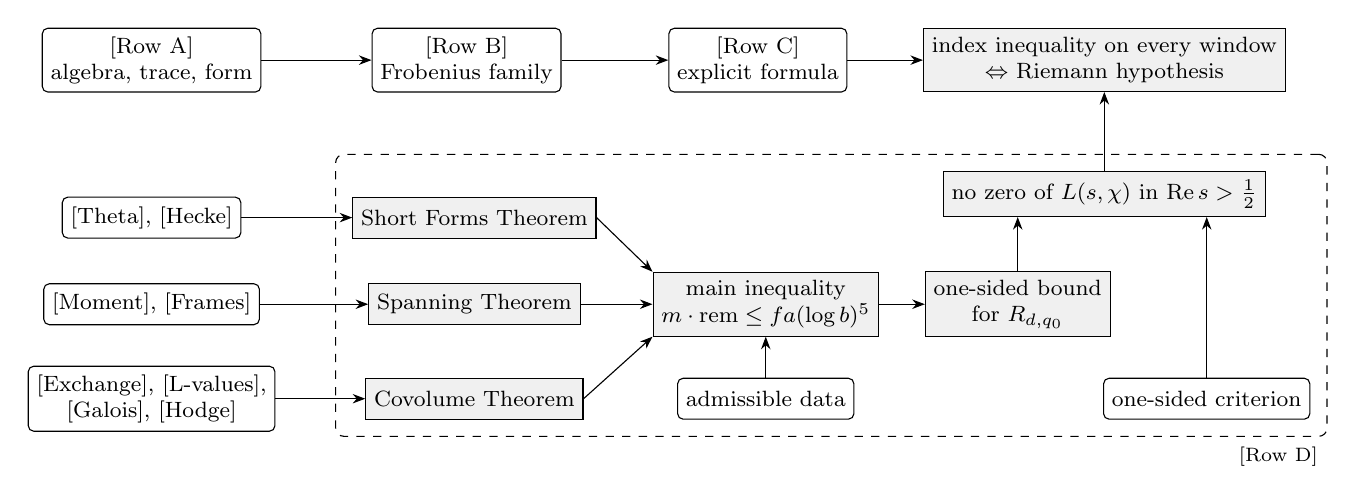
\begin{tikzpicture}[font=\footnotesize,
  box/.style={draw,rounded corners=2pt,align=center,inner sep=3pt,minimum height=5.2mm},
  res/.style={draw,align=center,inner sep=3pt,minimum height=5.2mm,fill=black!6},
  >={Stealth[length=1.6mm]}]
\node[box] (A) at (0.9,0) {[Row A]\\ algebra, trace, form};
\node[box] (B) at (4.9,0) {[Row B]\\ Frobenius family};
\node[box] (C) at (8.6,0) {[Row C]\\ explicit formula};
\node[res] (F) at (13.0,0) {index inequality on every window\\ $\Leftrightarrow$ Riemann hypothesis};
\draw[->] (A)--(B); \draw[->] (B)--(C); \draw[->] (C)--(F);
\node[box] (th) at (0.9,-2.0) {[Theta], [Hecke]};
\node[box] (mo) at (0.9,-3.1) {[Moment], [Frames]};
\node[box] (ex) at (0.9,-4.3) {[Exchange], [L-values],\\ {}[Galois], [Hodge]};
\node[res] (SF) at (5.0,-2.0) {Short Forms Theorem};
\node[res] (Sp) at (5.0,-3.1) {Spanning Theorem};
\node[res] (Cv) at (5.0,-4.3) {Covolume Theorem};
\draw[->] (th)--(SF); \draw[->] (mo)--(Sp); \draw[->] (ex)--(Cv);
\node[res] (MI) at (8.7,-3.1) {main inequality\\ $m\cdot\mathrm{rem}\le fa(\log b)^5$};
\draw[->] (SF.east)--(MI.north west); \draw[->] (Sp)--(MI); \draw[->] (Cv.east)--(MI.south west);
\node[box] (da) at (8.7,-4.3) {admissible data};
\draw[->] (da)--(MI);
\node[res] (OS) at (11.9,-3.1) {one-sided bound\\ for $R_{d,q_0}$};
\draw[->] (MI)--(OS);
\node[box] (cr) at (14.3,-4.3) {one-sided criterion};
\node[res] (G) at (13.0,-1.7) {no zero of $L(s,\chi)$ in $\Rel s>\frac12$};
\draw[->] (OS.north)--(OS.north |- G.south);
\draw[->] (cr.north)--(cr.north |- G.south);
\draw[->] (G)--(F);
\node[draw,dashed,rounded corners=3pt,inner sep=6pt,fit=(SF)(Cv)(MI)(OS)(da)(cr)(G)] (D) {};
\node[anchor=north east,font=\scriptsize] at (D.south east) {[Row D]};
\end{tikzpicture}
\caption{Dependencies. Rounded boxes are papers or constructions, shaded boxes are statements.
The dashed frame encloses what is proved in \cite{P46}, given the propositions proved in the
companions; the top box on the right is also in \cite{P46}.}\label{fig:deps}
\end{figure}

A reader interested in the analogy with Weil's proof may read \cite{P43}, \cite{P44} and
\cite{Paper45} in order; each begins by recalling what it takes from the preceding ones, and the
introduction of \cite{P46} and its section on the radial trace then suffice to see the index
inequality and its equivalence with the Riemann hypothesis. A reader interested in the proof
may start directly with \cite{P46}: the sections on the criterion, on the admissible data and
on the main inequality are elementary and complete in themselves, and they reduce everything to
the three theorems. The automorphic section of \cite{P46} states these, explains the mechanism
in more detail than we have done here, and deduces them from the propositions of the
companions. Among the companions, \cite{P49} is best read first, since the others use its
foundations; after it, \cite{P50}, the pair \cite{P51}, \cite{P52}, and the group
\cite{P53}, \cite{P54}, \cite{P55}, \cite{P56} can be read independently of one another, the
last group in that order; that group uses from \cite{P51} only the equality of multiplicities.

\section{Conclusion}\label{sec:conclusion}
The chain is complete. The correspondence algebra, its trace and its two Tate functionals are
built in \cite{P43}; the arithmetic family whose contacts with the diagonal are
$\Lambda(n)/\sqrt n$ in \cite{P44}; the trace is Weil's explicit formula by \cite{Paper45}; and
in \cite{P46}, with \cite{P49}--\cite{P56}, the criterion, the data and the three theorems
give the main inequality, the one-sided bound for the prime sum, and from it the absence of
zeros of every Dirichlet $L$-function in $\Rel s>\tfrac12$. I assert, on my own responsibility,
that with this chain the generalised Riemann hypothesis for Dirichlet $L$-functions is proved,
and with it the Riemann hypothesis. In the terms of the four rows, the index inequality holds
on every window: what Weil's proof does for a curve by means of the geometry of a surface is
done for $\operatorname{Spec}\Z$ by other means, and the positivity that the first three rows
leave open is true.

\subsection*{Acknowledgement}
Two things must be said about L.~Alpoge, and I wish to say them clearly. The first is that his
work is, by itself, a complete route to the generalised Riemann hypothesis for Dirichlet
$L$-functions and to the Riemann hypothesis: it is the formally verified proof
\cite{CharacterFamily}, and it owes nothing to the constructions of this series. The second
is that his work is, in addition, the input that closes the path taken in this series, which is
to carry out Weil's proof over $\operatorname{Spec}\Z$. The Short Forms Theorem, the Spanning
Theorem and the Covolume Theorem are our formulation: the division of the argument into these
three statements, and their names, are ours, and so is the writing of their proofs as
mathematics on paper. The mathematics they organise, and the way from them to the zero-free
half-plane, are his. Rows~A, B and~C, and the study of the radial form in Row~D, lay out a
path and identify the inequality at its end; they do not prove it. It is his argument, in the
form of these three theorems, that closes the path. I record this debt with gratitude.

\begin{thebibliography}{L-values}
\bibitem[Row A]{P43} D.~A.~Trejo Pizzo,
\emph{A correspondence algebra and the Weil distribution on semilocal idele
class groups}, preprint, 2026, \url{https://github.com/dtrejopizzo/riemann/tree/main/04-papers/43-row-a-correspondence-algebra}.
\bibitem[Row B]{P44} D.~A.~Trejo Pizzo,
\emph{An arithmetic Frobenius family on semilocal idele class groups},
preprint, 2026, \url{https://github.com/dtrejopizzo/riemann/tree/main/04-papers/44-row-b-arithmetic-family}.
\bibitem[Row C]{Paper45} D.~A.~Trejo Pizzo, \emph{An explicit formula for the trace on semilocal idele class groups}, preprint, 2026, \url{https://github.com/dtrejopizzo/riemann/tree/main/04-papers/45-row-c-explicit-formula}.
\bibitem[Row D]{P46} D.~A.~Trejo Pizzo, \emph{The sign of the radial intersection form on the idele class group}, preprint, 2026, \url{https://github.com/dtrejopizzo/riemann/tree/main/04-papers/46-row-d-sign-radial-intersection-form}.
\bibitem[Theta]{P49} D.~A.~Trejo Pizzo, \emph{The Short Forms Theorem: theta lifts, complex multiplication and divisibility}, preprint, 2026, \url{https://github.com/dtrejopizzo/riemann/tree/main/04-papers/49-short-forms-theorem-theta-lifts-complex-multiplication}.
\bibitem[Hecke]{P50} D.~A.~Trejo Pizzo, \emph{Elementary divisors of an edge Hecke operator on a Frobenius cycle}, preprint, 2026, \url{https://github.com/dtrejopizzo/riemann/tree/main/04-papers/50-elementary-divisors-edge-hecke-operator}.
\bibitem[Moment]{P51} D.~A.~Trejo Pizzo, \emph{The Spanning Theorem: the second moment of a Poincar\'e map}, preprint, 2026, \url{https://github.com/dtrejopizzo/riemann/tree/main/04-papers/51-spanning-theorem-second-moment-poincare-map}.
\bibitem[Frames]{P52} D.~A.~Trejo Pizzo, \emph{The Spanning Theorem: sieve systems at the real and finite places and Siegel's step}, preprint, 2026, \url{https://github.com/dtrejopizzo/riemann/tree/main/04-papers/52-sieve-systems-siegel-step}.
\bibitem[Exchange]{P53} D.~A.~Trejo Pizzo, \emph{The Covolume Theorem: exchange identities and the determinant of a chain of theta lifts}, preprint, 2026, \url{https://github.com/dtrejopizzo/riemann/tree/main/04-papers/53-covolume-theorem-exchange-identities-chain-determinant}.
\bibitem[L-values]{P54} D.~A.~Trejo Pizzo, \emph{The Covolume Theorem: one theta lift, Hecke $L$-values and test forms of least valuation}, preprint, 2026, \url{https://github.com/dtrejopizzo/riemann/tree/main/04-papers/54-covolume-theorem-one-theta-lift-hecke-l-values}.
\bibitem[Galois]{P55} D.~A.~Trejo Pizzo, \emph{The Covolume Theorem: regular families of twists, Selmer groups and Ribet's method}, preprint, 2026, \url{https://github.com/dtrejopizzo/riemann/tree/main/04-papers/55-covolume-theorem-regular-families-of-twists}.
\bibitem[Hodge]{P56} D.~A.~Trejo Pizzo, \emph{Explicit cup exponents for local Galois representations beyond the Fontaine--Laffaille range}, preprint, 2026, \url{https://github.com/dtrejopizzo/riemann/tree/main/04-papers/56-explicit-cup-exponents-local-galois-representations}.
\bibitem{CharacterFamily} L.~Alpoge, Lean~4 formalisation of the character-family argument
for Dirichlet $L$-functions, source archive in fourteen parts, November 2026,
\url{https://alpo.ge/lean.tar.gz.part01} (first part).
\bibitem{BannaiKobayashi} K.~Bannai and S.~Kobayashi, \emph{Algebraic theta functions and the
$p$-adic interpolation of Eisenstein--Kronecker numbers}, Duke Math.\ J.\ \textbf{153} (2010),
229--295.
\bibitem{Bombieri2000} E.~Bombieri, \emph{Remarks on Weil's quadratic functional in the theory of
prime numbers, I}, Atti Accad.~Naz.~Lincei Cl.~Sci.~Fis.~Mat.~Natur.~Rend.~Lincei (9) Mat.~Appl.
\textbf{11} (2000), no.~3, 183--233.
\bibitem{Chellali} M.~Chellali, \emph{Congruences entre nombres de Bernoulli--Hurwitz dans le cas
supersingulier}, J.\ Number Theory \textbf{35} (1990), 157--179.
\bibitem{Connes99} A.~Connes, \emph{Trace formula in noncommutative geometry and the zeros of
the Riemann zeta function}, Selecta Math.\ (N.S.) \textbf{5} (1999), 29--106.
\bibitem{ConnesConsani2021} A.~Connes and C.~Consani, \emph{Weil positivity and trace formula, the archimedean place}, Selecta Math.\ (N.S.) \textbf{27} (2021), no.~4, Paper No.~77; arXiv:2006.13771.
\bibitem{CCM} A.~Connes, C.~Consani and M.~Marcolli, \emph{The Weil proof and the geometry
of the ad\`eles class space}, in: Algebra, Arithmetic, and Geometry: in honor
of Yu.~I.~Manin, Vol.~I, Progr.\ Math.\ \textbf{269}, Birkh\"auser, Boston,
2009, 339--405, arXiv:math/0703392.
\bibitem{Davenport} H.~Davenport, \emph{Multiplicative Number Theory}, 3rd ed., revised by
H.~L.~Montgomery, Graduate Texts in Mathematics \textbf{74}, Springer, New York, 2000.
\bibitem{GrossAMF} B.~H.~Gross, \emph{Algebraic modular forms}, Israel J.\ Math.\ \textbf{113}
(1999), 61--93.
\bibitem{HeathBrown1995} D.~R.~Heath-Brown, \emph{A mean value estimate for real character
sums}, Acta Arith.\ \textbf{72} (1995), no.~3, 235--275.
\bibitem{KatzDivisibilities} N.~M.~Katz, \emph{Divisibilities, congruences, and Cartier duality},
J.\ Fac.\ Sci.\ Univ.\ Tokyo Sect.\ IA Math.\ \textbf{28} (1981), 667--678.
\bibitem{MV} H.~L.~Montgomery and R.~C.~Vaughan, \emph{Multiplicative Number Theory I.
Classical Theory}, Cambridge Studies in Advanced Mathematics \textbf{97}, Cambridge
Univ.~Press, 2007.
\bibitem{Weil1948} A.~Weil, \emph{Sur les courbes alg\'ebriques et les vari\'et\'es qui s'en
d\'eduisent}, Actualit\'es Sci.\ Ind.\ \textbf{1041}, Hermann, Paris, 1948.
\bibitem{Weil52} A.~Weil, \emph{Sur les ``formules explicites'' de la th\'eorie des nombres
premiers}, Comm.~S\'em.~Math.~Univ.~Lund (1952), 252--265.
\bibitem{Yoshida1992} H.~Yoshida, \emph{On Hermitian forms attached to zeta functions}, in:
\emph{Zeta Functions in Geometry}, Adv.~Stud.~Pure Math.~\textbf{21}, Kinokuniya, Tokyo, 1992, 281--325.
\end{thebibliography}
\end{document}
